% Based on http://texwelt.de/wissen/fragen/13193/kommentierter-sitzplan-mit-tikz

\documentclass{scrartcl}
\usepackage[a4paper, landscape, total={25cm, 18cm}]{geometry}
\usepackage{fontspec}
\usepackage{bbding}
\usepackage{graphicx}
\usepackage{ifthen}
\usepackage{tikz}
\usetikzlibrary{matrix}

\tikzset{
  platz/.style={
    draw,
    text width=3cm,
    align=center,
    minimum height=3.5\baselineskip
}}

\thispagestyle{empty}

\begin{document}
\begin{center}
{\Large \textbf{Sitzplan}}
\par\medskip
\noindent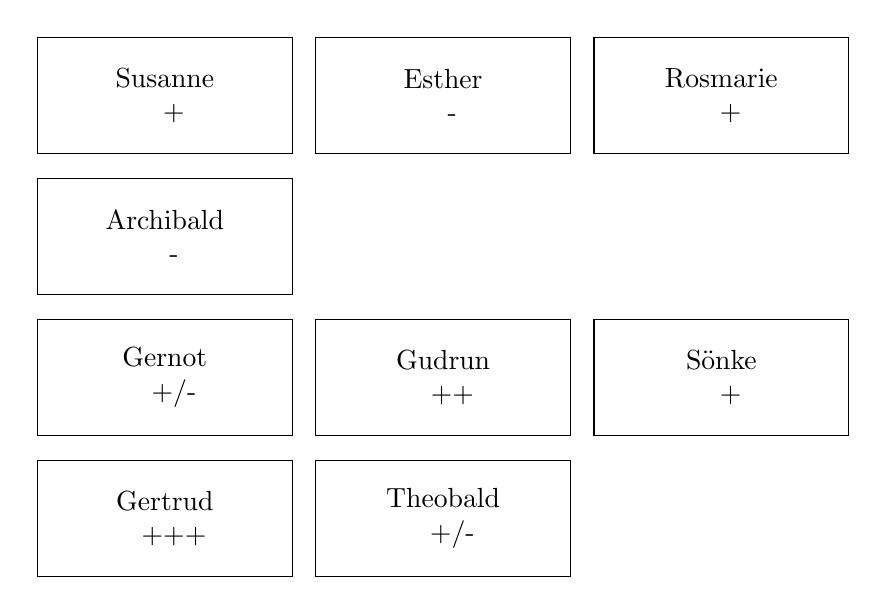
\begin{tikzpicture}
  \matrix(sitzplan)[
      matrix of nodes,
      row sep=3mm,
      column sep=-\pgflinewidth,
%      nodes in empty cells,
      nodes={platz,anchor=center}
    ]{{Susanne\\{\scalebox{.7}{\rotatebox[x=0mm, y=4mm]{-90}{\HandLeft}}}{\scalebox{.7}{\rotatebox[x=0mm, y=4mm]{-90}{\HandLeft}}}{\scalebox{.7}{\rotatebox[x=0mm, y=4mm]{-90}{\HandLeft}}}~~+}&[3mm]{Esther\\{\scalebox{.7}{\rotatebox[x=0mm, y=4mm]{-90}{\HandLeft}}}{\scalebox{.7}{\rotatebox[x=0mm, y=4mm]{-90}{\HandLeft}}}{\scalebox{.7}{\rotatebox[x=0mm, y=4mm]{-90}{\HandLeft}}}{\scalebox{.7}{\rotatebox[x=0mm, y=4mm]{-90}{\HandLeft}}}~~-}&[3mm]{Rosmarie\\{\scalebox{.7}{\rotatebox[x=0mm, y=4mm]{-90}{\HandLeft}}}~~+}\\
{Archibald\\{\scalebox{.7}{\rotatebox[x=0mm, y=4mm]{-90}{\HandLeft}}}{\scalebox{.7}{\rotatebox[x=0mm, y=4mm]{-90}{\HandLeft}}}~~-}&&\\
{Gernot\\{\scalebox{.7}{\rotatebox[x=0mm, y=4mm]{-90}{\HandLeft}}}{\scalebox{.7}{\rotatebox[x=0mm, y=4mm]{-90}{\HandLeft}}}{\scalebox{.7}{\rotatebox[x=0mm, y=4mm]{-90}{\HandLeft}}}~~+/-}&{Gudrun\\{\scalebox{.7}{\rotatebox[x=0mm, y=4mm]{-90}{\HandLeft}}}{\scalebox{.7}{\rotatebox[x=0mm, y=4mm]{-90}{\HandLeft}}}~~++}&{Sönke\\{\scalebox{.7}{\rotatebox[x=0mm, y=4mm]{-90}{\HandLeft}}}{\scalebox{.7}{\rotatebox[x=0mm, y=4mm]{-90}{\HandLeft}}}{\scalebox{.7}{\rotatebox[x=0mm, y=4mm]{-90}{\HandLeft}}}~~+}\\
{Gertrud\\~~+++}&{Theobald\\{\scalebox{.7}{\rotatebox[x=0mm, y=4mm]{-90}{\HandLeft}}}~~+/-}&\\
};
\end{tikzpicture}

\end{center}
\end{document}
